% !TEX encoding = UTF-8
% !TEX TS-program = pdflatex
% !TEX root = ../elsarticle-template-num.tex
% !TEX spellcheck = en-EN

%************************************************
\section{Method}
\label{sec:method}
%************************************************
%\section{Method}
%\label{sec:method}
%************************************************

%%%\lipsum[1]
%%\begin{equation}
\label{eq:emc}
e = mc^2
\end{equation}





\subsection{Discrete element method}
\label{subsec:dem}
The $DEM$ is based on a relatively elementary idea. For each particle i inside
the domain it follows the course and calculate the force of that exerts on particle j
by integrating Newton' second law:
\begin{equation}
m \ddot{x}_{ij} + c \dot{x}_{ij} + k x_{ij} =  F_{ij} .
\label{equ:newtonlaw}
\end{equation}

and the position and orientation equations.
The main forces interested are: gravitation, contact forces due to collisions,
solid-solid interactions such as electrostatic, Van der Waals, cohesive forces
and fluid-solid interactions in multiphase flows.

For the raw materials used in this work \cite{RefWorks:145} suggested using the non-linear Hertzian model without cohesion for the particle-particle and particle-wall contacts.\\
This granular model uses the following formula for the force between two granular particles (Eq. \ref{eq:forceij}):
\begin{equation}
 F_{ij} = 
\begin{cases}
F_{n,ij} + F_{t,ij} = \left( k_n \delta_{n,ij} + \gamma_n v_{n,ij} \right) + \left( k_t \delta_{t,ij} + \gamma_t v_{t,ij} \right) & \text{if } r < d ,\\
0    & \text{if } r > d ,\\
\end{cases}
 \label{eq:forceij}
\end{equation}

while the tangential force component is truncated to fulfill
\begin{equation}
F_{t,ij} \leq \mu_s F_{n,ij},
 \label{eq:force_t}
\end{equation}

Both the normal and the tangential force comprise two terms, a spring force and a damping force. The shear force is a "history" effect that accounts for the tangential displacement 
("tangential overlap") between the particles for the duration of contact. \\

The $k_n$, $k_t$, $\gamma_n$, and $\gamma_t$ coefficients are calculated from the material properties as follows:
\begin{equation}
\begin{aligned}
	k_n &= \frac{4}{3} E_{eq} \sqrt{R_{eq} \xi_n} ,\\
	\gamma_n &= 2 \sqrt{\frac{5}{6}} \beta \sqrt{S_n m_{eq}} ,\\
	k_t &= 8 G_{eq} \sqrt{R_{eq}} \xi_n ,\\
	\gamma_t &= 2 \sqrt{\frac{5}{6}} \beta \sqrt{S_t m_{eq}} .
\end{aligned}
\label{eq:hertz}
\end{equation}

In addition to the equations \ref{eq:hertz} the following relations (Eqns. \ref{eq:equivProp2}) are required:
\begin{equation}
\begin{aligned}
 \frac{1}{E_{eq}} & = \frac{1-\nu_i^2}{E_i} + \frac{1-\nu_j^2}{E_j} ,\\
 \frac{1}{G_{eq}} & = \frac{2(2+\nu_i)(1-\nu_i)}{E_i} + \frac{2(2+\nu_j)(1-\nu_j)}{E_j} ,\\
 \frac{1}{R_{eq}} &= \frac{1}{R_i} + \frac{1}{R_j} ,\\
 \frac{1}{m_{eq}} &= \frac{1}{m_i} + \frac{1}{m_j} ,\\
 \beta & = \frac{\ln(e)}{\sqrt{ln^2(e)+\pi^2}} ,\\
 S_n & = 2 E_{eq} \sqrt{R_{eq} \delta_n} ,\\
 S_t & = 8 G_{eq} \sqrt{R_{eq} \delta_n} ,\\
 k_r & = k_t R_{eq}^2 .\\
\end{aligned}
\label{eq:equivProp2}
\end{equation}


The coefficient of sliding friction for coarse round particles is a critical
parameter describing inter-particle friction in medium to dense granular flows simulations.
It is proportional to the torque counteracting the rotation of the particle and defined as (Eq. \ref{equ:mur}):
\begin{equation}
 \mu_r =  \tan(\iota) .
\label{equ:mur}
\end{equation}

The $\mu_r$ parameter enters the equations according to the elasto-rolling resistance model presented by \cite{RefWorks:87} and \cite{RefWorks:131}, also used by \cite{RefWorks:147}, 
based on the work of \cite{RefWorks:143}(and in contrast to \cite{RefWorks:144}). The model is called EPSD2 in LIGGGHTS.
This is appropriate for the one way rolling cases as well as the cycling rolling ones.
The total rolling resistance torque is (Eq. \ref{eq:mrtm}):
\begin{equation}
\begin{aligned}
M_r &= M_r^k ,\\
M_{r,ti+\Delta ti}^k &= M_{r,ti}^k - k_r \Delta \theta_r ,\\
\lvert{M_{r,ti+\Delta ti}^k}\rvert & \leq M_r^m = \mu_r R_{eq} F_n .\\
\end{aligned}
 \label{eq:mrtm}
\end{equation}


Given these equations, completely defining a dry material for DEM simulations requires these data:
\begin{itemize}
\item{the radius of the particles ($R$);}
\item{the Young's modulus ($E$) and the Poisson's coefficient ($\nu$);}
\item{the particle density ($\rho_p$) and the coefficient of restitution ($e$);}
\item{the coefficients of sliding ($\mu_s$) and rolling ($\mu_r$) friction.}
\end{itemize}


Further details on the method can be found in \cite{RefWorks:133}.





\subsection{Artificial Neural Networks}
\label{subsec:ann}

An Artificial Neural Network (NN) is a powerful modellization technique, based
on non-linear functions (Haykin \cite{RefWorks:158}). In this paper, we first use them to fit the DEM
numerical simulation data, and then to process vast amount of parameters combinations.
NN original idea is directly borrowed from human brain design, with neurons and
synapses.
There are divers types of NN, remarkably the Feedforward (FF) and the Radial
basis function (RBF). For FF-NN, considerable
amount of traning algorithms are available. The most common are based on
backpropagation: Levenberg-Marquardt, Bayesian regulation and scaled conjugate
gradient. Following the best practice suggested by Vaferi et al. \cite{RefWorks:150}
\textit{FF Multilayer Perceptron Neural Networks (MLPNN)} have been
handled. They map combinations of input data into convenient outputs (fitting).
Each processing units or node (neuron) possesses a nonlinear activation
function. Together, they are interconnected into layers, also linked together.
To recognize not linearly separable data the standard 
linear perceptron $NN$ has been modified into $MLPNN$.
Their trustworthiness, together with a backpropagation reinforcement
learning training algorithm (scaled conjugate gradient), has been widely
demonstrated in the literature, see Haykin \cite{RefWorks:158}.
Several scientists \cite{RefWorks:161, RefWorks:166, RefWorks:167, RefWorks:168, RefWorks:169,
RefWorks:170} have operated $NN$ to model materials mechanical properties.
In fact, $MLPNN$ are built with three different layers.
The input layer has a number of neurons equal to the number of different inputs
of the network. Similarly for a Best practice also demands to establish the
most appropriate number of neurons inside the hidden layer of each $NN$.
As in literature, this goal has been achieved by first excluding 15\% of the
simulations from th  training processes.
%\lipsum[1]
%\begin{equation}
\begin{aligned}
M_r &= M_r^k ,\\
M_{r,ti+\Delta ti}^k &= M_{r,ti}^k - k_r \Delta \theta_r ,\\
\lvert{M_{r,ti+\Delta ti}^k}\rvert & \leq M_r^m = \mu_r R_{eq} F_n .\\
\end{aligned}
 \label{eq:mrtm}
\end{equation}


\subsection{Experimental setup}
\label{subsec:experimentalsetup}

The first step of the procedure was using a SRSCT (see \cite{RefWorks:142}) to characterize particle flow properties, especially the complete yield locus.
A representative sample of bulk solid was placed in a shear cell of specified dimensions ($external ~ radius = 100 ~ mm$, $internal ~ radius = 50 ~ mm$). 
\begin{figure}[!htb] 
\centering 
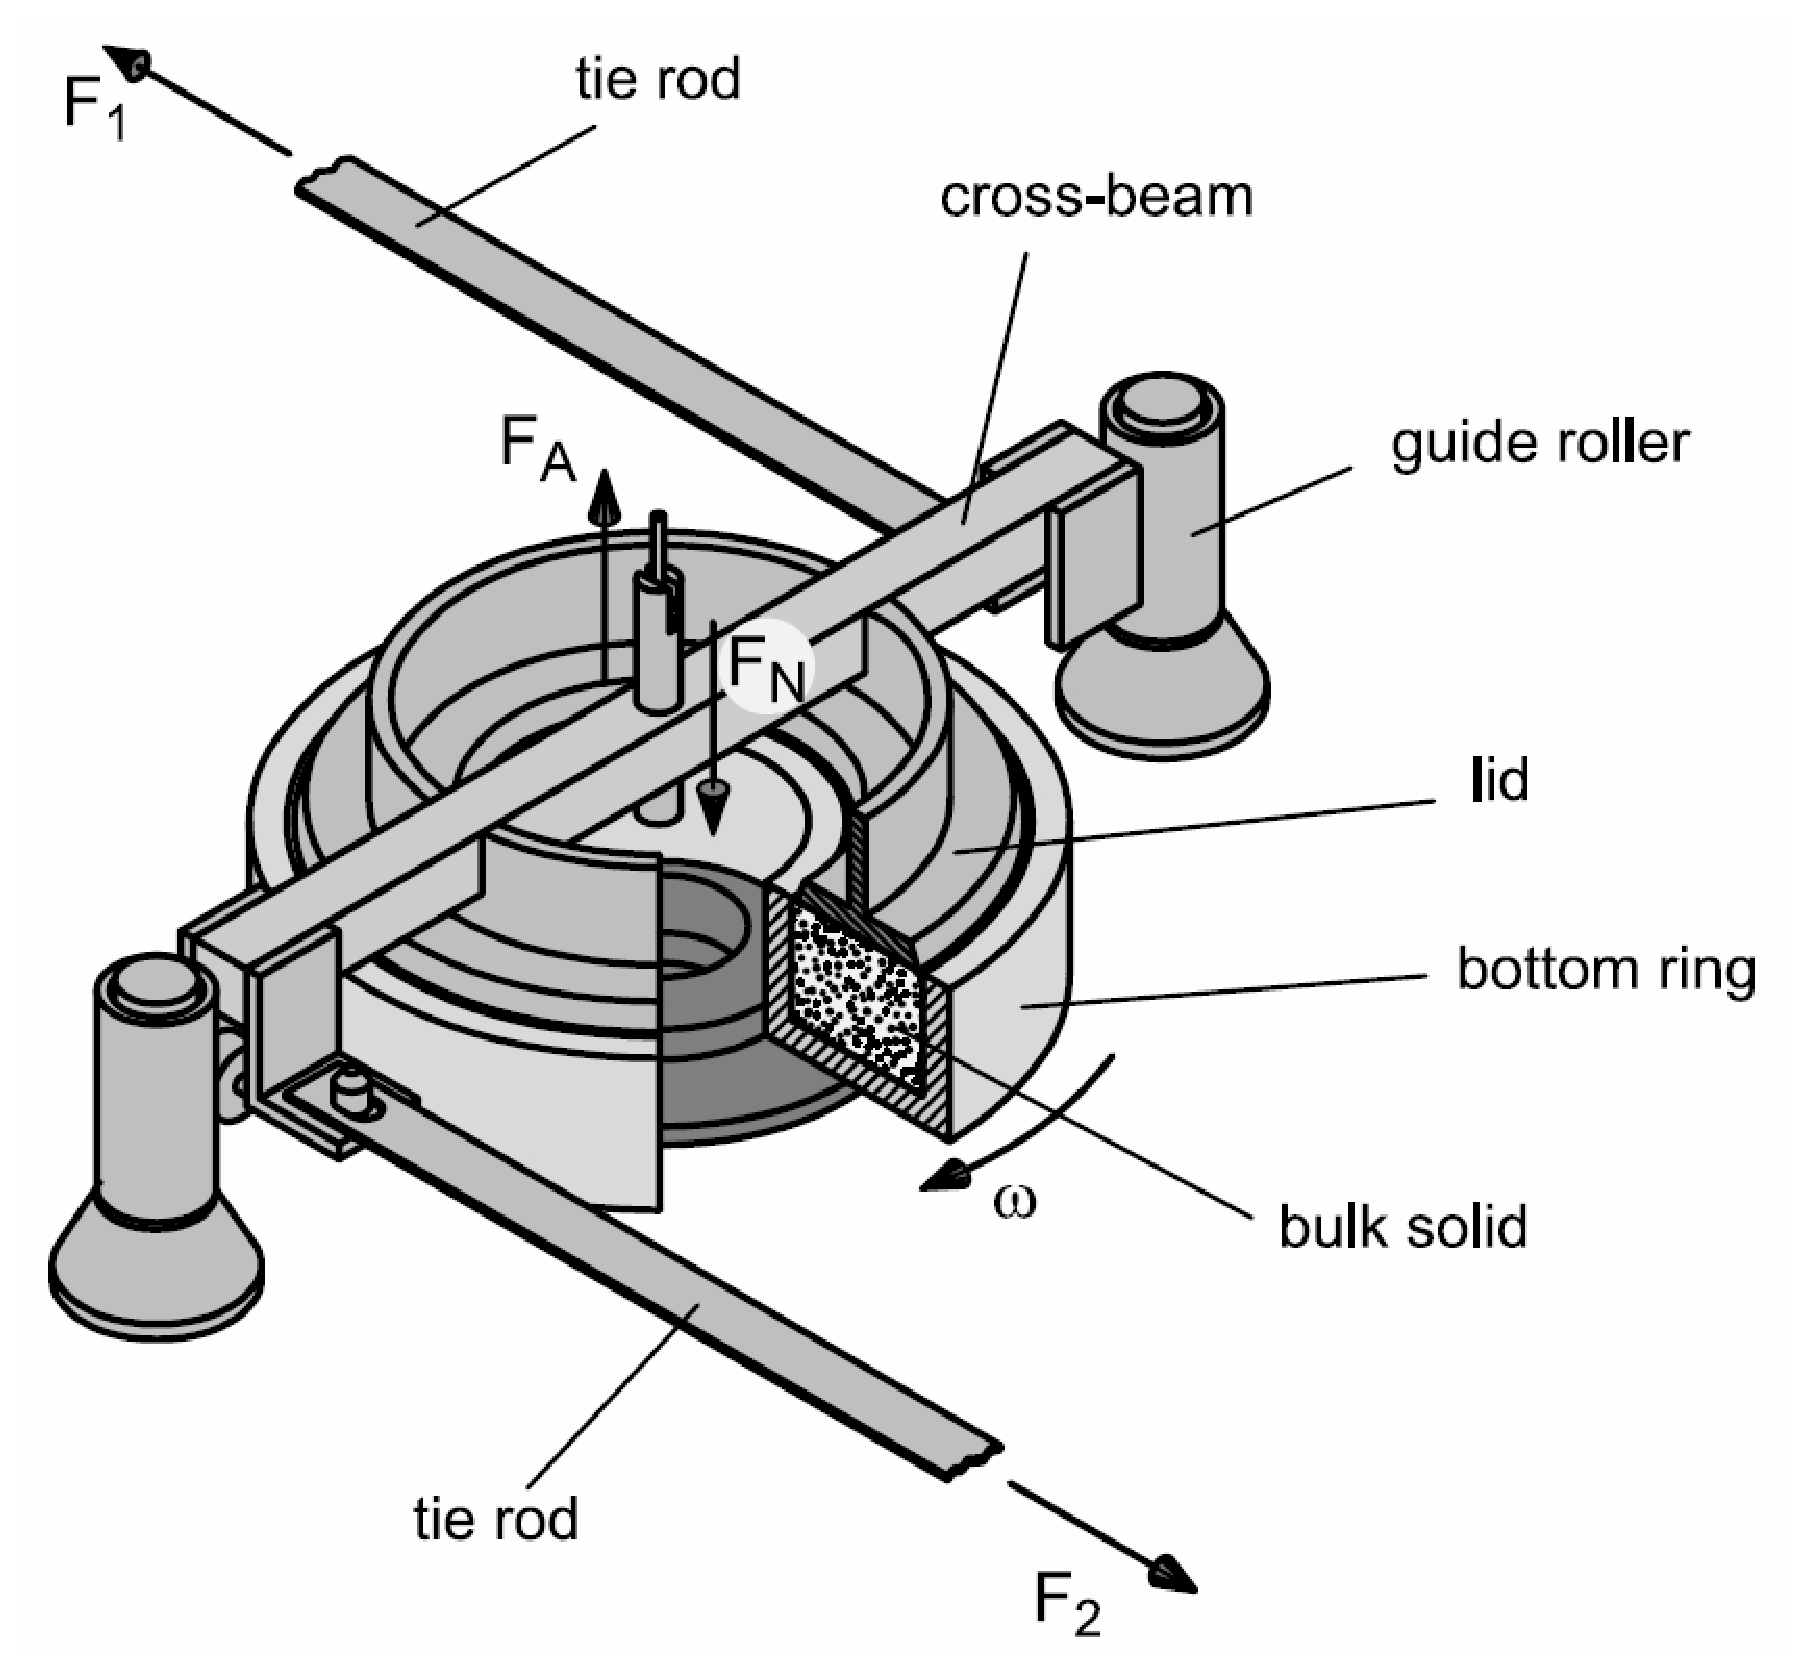
\includegraphics[width=.8\textwidth]{images/original/01srsct} 
\caption[Schulze ring shear cell tester]{Schulze ring shear cell tester
experimental layout, Schulze \cite{RefWorks:118}}
\label{fig:01srsct} 
\end{figure}


% \begin{figure}[htp]
%     \centering
%     
\includegraphics[width=.2\textwidth]{images/vitae/lbenvenuti}
%     \caption{OpenMP, MPI, MPI/OpenMP Hybrid runs of Box in a box testcase on 32
%     cores. The OpenMP-only run suffers from limited memory bandwidth in
%     memory-bound algorithms inside of the Modify section of the code. MPI-only has
%     low averaged runtimes for each section, but a very large Other timing, which
%     hints for a large amount of load-imbalance. Hybrid timings are a bit worse
%     on average, but because of better balancing, processes have lower wait times
%     inside of Other timing.}
% 	\label{fig:boxInBoxComparison}

A normal load was applied to the cover, and the specimen was pre-sheared  until a steady-state shear value was reached.
 The steady-state flow horizontal stress (Fig. \ref{fig:02srsctdiagram}) is
called pre-shear stress ($\tau_{psh}$). Knowing the normal stress, it gives (Eq. \ref{eq:phi_ps}) the angle of internal friction of the pre-shear phase 
($\phi_{e-psh}$), our first flowability value \cite{RefWorks:118}:
\begin{equation}
\begin{aligned}
\phi_{e-psh} &= \arctan \left(\frac{\tau_{psh}}{\sigma_{n,psh}} \right) ,\\
\mu_{psh} &=\tan(\phi_{e-psh}) .
\end{aligned}
 \label{eq:phi_ps}
\end{equation}
 
\begin{figure}[!htb] 
\centering 
\includegraphics[width=.8\textwidth]{images/original/02srsctdiagram.eps} 
\caption{Schulze ring shear cell tester diagram \cite{RefWorks:118}}
\label{fig:02srsctdiagram} 
\end{figure}


% \begin{figure}[htp]
%     \centering
%     
\includegraphics[width=.2\textwidth]{images/vitae/lbenvenuti}
%     \caption{OpenMP, MPI, MPI/OpenMP Hybrid runs of Box in a box testcase on 32
%     cores. The OpenMP-only run suffers from limited memory bandwidth in
%     memory-bound algorithms inside of the Modify section of the code. MPI-only has
%     low averaged runtimes for each section, but a very large Other timing, which
%     hints for a large amount of load-imbalance. Hybrid timings are a bit worse
%     on average, but because of better balancing, processes have lower wait times
%     inside of Other timing.}
% 	\label{fig:boxInBoxComparison}

The normal stress and the angular velocity were then immediately reduced to zero. 
Subsequently, the specimen was sheared under a fraction of the first normal load until the shear force reached a maximum and began to decrease. 
Both the pre-shear and shear phases were executed at constant velocity. We define the horizontal stress during the shear force peak as maximum shear stress, 
thus obtaining (Eq. \ref{eq:phi_s})\cite{RefWorks:118}:
\begin{equation}
\begin{aligned}
\phi_{e-sh} &= \arctan \left(\frac{\tau_{sh}}{\sigma_{n,sh}} \right) ,\\
\mu_{sh} &= \tan(\phi_{e-sh}) .
\end{aligned}
 \label{eq:phi_s}
\end{equation}
 
Each experiment was performed on a fresh material sample. \\


